\section{Experimental results} \label{sec:exp}\label{sec:gsetting}

In this section, the experimental results for the two proposed instances are presented. First, the Deep-ADV Multi-Class Classification (D-ADV-MC) instance has been validated with the INRIA, CAVIAR and BEHAVE datasets \cite{blunsden2010behave,fisher2004pets04}. On the other hand, the Deep-ADV One-Class Classification (D-ADV-OC) has been tested with the Ped 1, Ped 2 \cite{mahadevan2010anomaly} and Avenue \cite{lu2013abnormal} datasets. 

The general experimentation configuration for both instances are as follows:
\begin{itemize}
    \item Size of the cells that conform the images $LRF$ and $UDF$ is 224 x 224.
    \item The CNN based image classifier is the ResNet50. 
    \item The images $LRF$ and $UDF$ provided by the D-ADV representation stage have been normalized as input of the ResNet50 to the range between 0 and 1 by dividing each cell (pixel) by the maximum value of each component (L,R,U,D and F). 
\end{itemize}

The CNN based image classifier has been trained using transfer learning from the Imagenet dataset in three steps. First, only the last layer has been trained with the specific labels of the corresponding dataset. Second, the first 139 layers of the activity recognition module has been trained as a domain adaptation solution from the RGB to the $LRF$ and $UDF$ domain. Finally, from the top layer to the layer 249 is finally trained.
\subsection{Multi-Class Classification results}\label{sec:exp:mc}

A 10-fold cross validation has been used to calculate the performance of the architecture for the different datasets. Moreover, 25\% of the training data in each fold has been used for the validation set. Specifically, the performance of the D-ADV has been evaluated 
using the sensitivity, specificity (see Table \ref{tab:frame_sequence}) and the AUC and ROC curves (see Figure \ref{fig:fig_behave}, Figure \ref{fig:fig_inria} and Figure \ref{fig:fig_corridor}). These values have been calculated for frames and for sequences. That is, the performance per frame is calculated according to the prediction made on each individual frame independently of the sequence. The performance per sequence is calculated according to the prediction made for all the frames in the sequence. For this, the prediction of the sequence is the one corresponding to the one corresponding to at least 80\% of the frames of the sequence. Finally, in order to evaluate the ability of the representation to synthesize the information extracted from the scene, two different values for the windowsize ($ws$) parameter have been tested: 10 and 40 (i.e. ~0.5 sec. and 2 sec.).  

The per-frame performance results with a window size ($ws$) of 10 reach according to the sensitivity and specificity, for the INRIA dataset, 71.70\% and 84.85\% on average, 91.47\% and 94.51\% for BEHAVE dataset, while 78.18\% and 87.12\% respectively for the CAVIAR (corridor) dataset. Using a larger window size (i.e. $ws$ of 40), the results are improved in the three datasets, obtaining 89.93\% and 95.65\% (senditivity and specificity) for INRIA, 92.55\% and 94.79\%  for BEHAVE dataset, and 79.00\% and 88.88\% for the CAVIAR dataset (see \ref{tab:frame_sequence}). 

In terms of performance per sequence, D-ADV achieves very high results. Considering a window size of 10, for the INRIA dataset, a total of 91.67\% of sensitivity and 95.83\% of specificity is achieved, while 95.07\% and 95.52\%  for the BEHAVE dataset, 80.00\% and 93,06 respectively for CAVIAR dataset. Again, the results considering a larger value for the window size ($ws=40$) are improved achieving the best ones. On average, 95.83\% of sensitivity and 97.92\% of specificity for the INRIA dataset, 95.52\% and 95.70\% respectively for the BEHAVE dataset and, finally, 80.58\% and 94,27 for CAVIAR dataset.


Finally, the D-ADV architecture is compared with the methods proposed in \cite{azorin2016}, \cite{cho2015group}, \cite{zhang2012recognizing}, \cite{munch2012supporting}, \cite{yin2013small} considering the seven classes of the BEHAVE dataset. Only \cite{cho2015group} and our previous work (GADV) consider the seven classes as well. The rest of the works use a subset of four classes. Table \ref{tab:ComparisonBEHAVE} shows the comparison of the sensitivity results. As we can see, our proposal, D-ADV, achieves in average the best results outperforming all compared methods.
%inicio tabla
\begin{table*}
	\centering
	\caption{Comparison of results with datasets (INRIA, BEHAVE, CAVIAR) calculated for frame and sequence with windowsize ($ws$) values 10 and 40.}
	\label{tab:frame_sequence}
	\resizebox{0.99\textwidth}{!}{\begin{tabular}{|c|l|c|c|c|c|c|c|c|c|} 
	\cline{3-10}
	\multicolumn{1}{l}{}               &                   & \multicolumn{4}{c|}{\textbf{Frame} }                                          & \multicolumn{4}{c|}{\textbf{Sequence} }                                        \\ 
	\cline{3-10}
	\multicolumn{1}{l}{}               &                   & \multicolumn{2}{c|}{\textbf{$ws=10$} }     & \multicolumn{2}{c|}{\textbf{$ws=40$} }     & \multicolumn{2}{c|}{\textbf{$ws=10$} }     & \multicolumn{2}{c|}{\textbf{$ws=40$} }      \\ 
	\hline
	\textbf{Dataset}                   & \textbf{Class}    & Sensitivity       & Specificity       & Sensitivity       & Specificity       & Sensitivity       & Specificity       & Sensitivity       & Specificity        \\ 
	\hline
	\multirow{4}{*}{Inria}             & Fighting          & 82.84\%           & 76.46\%           & 95.48\%           & 94.00\%           & 100.00\%          & 100.00\%          & 100.00\%          & 100.00\%           \\ 
	\cline{2-10}
	& Leaving           & 95.87\%           & 94.79\%           & 99.68\%           & 99.74\%           & 87.50\%           & 93.75\%           & 100.00\%          & 100.00\%           \\ 
	\cline{2-10}
	& Meeting           & 65.11\%           & 75.10\%           & 86.85\%           & 87.58\%           & 87.50\%           & 93.75\%           & 87.50\%           & 93.75\%            \\ 
	\cline{2-10}
	& \textbf{Overall}  & \textbf{71.70\%}  & \textbf{84.85\%}  & \textbf{89.93\%}  & \textbf{95.65\%}  & \textbf{91.67\%}  & \textbf{95.83\%}  & \textbf{95.83\%}  & \textbf{97.92\%}   \\ 
	\hline
	\multirow{7}{*}{Behave}            & Approach          & 90.88\%           & 92.45\%           & 92.02\%           & 92.68\%           & 93.94\%           & 92.08\%           & 93.94\%           & 95.05\%            \\ 
	\cline{2-10}
	& Split             & 92.58\%           & 93.23\%           & 95.18\%           & 93.92\%           & 97.14\%           & 95.96\%           & 97.14\%           & 96.97\%            \\ 
	\cline{2-10}
	& Fight             & 95.52\%           & 96.35\%           & 93.40\%           & 95.27\%           & 100.00\%          & 98.28\%           & 94.44\%           & 93.10\%            \\ 
	\cline{2-10}
	& InGroup           & 94.41\%           & 94.32\%           & 94.15\%           & 93.75\%           & 94.83\%           & 94.74\%           & 93.10\%           & 93.42\%            \\ 
	\cline{2-10}
	& RunTogheter       & 99.87\%           & 99.95\%           & 100.00\%          & 99.99\%           & 100.00\%          & 100.00\%          & 100.00\%          & 100.00\%           \\ 
	\cline{2-10}
	& WalkTogheter      & 84.12\%           & 88.30\%           & 87.92\%           & 90.82\%           & 92.31\%           & 88.41\%           & 96.92\%           & 94.20\%            \\ 
	\cline{2-10}
	& \textbf{Overall}  & \textbf{91.47\%}  & \textbf{94.51\%}  & \textbf{92.55\%}  & \textbf{94.79\%}  & \textbf{95.07\%}  & \textbf{95.52\%}  & \textbf{95.52\%}  & \textbf{95.70\%}   \\ 
	\hline
	\multirow{5}{*}{Caviar} & Meeting           & 87.59\%           & 86.25\%           &  90.58\%               & 90.47\%            & 88.24\%           & 93.18\%           &  94.12\%               & 100.00\%             \\ 
	\cline{2-10}
	& Shop-Enter        & 91.28\%           & 91.14\%           & 85.80\%                & 93.86\%               & 100.00\%          & 95.56\%           & 87.50\%              & 93.33\%            \\ 
	\cline{2-10}
	& Shop-Exit         & 81.21\%           & 87.10\%           & 83.63\%                & 85.82\%                & 90.00\%           & 95.12\%           & 90.00\%                 & 90.24\%                 \\ 
	\cline{2-10}
	& Walking           & 72.16\%           & 76.49\%           & 73.57\%                 & 75.17\%                & 65.96\%           & 78.57\%           & 68.09\%               & 78.57\%                  \\ 
	\cline{2-10}
	& \textbf{Overall}  & \textbf{78.18\%}  & \textbf{87.12\%}  & \textbf{79.00\%}         & \textbf{88.88\%}         & \textbf{80.00\%}  & \textbf{93.06\%}  & \textbf{80.00\%}         & \textbf{93.06\%}          \\
	\hline
	\end{tabular}}
\end{table*}
% fin tabla
\begin{figure*}
\begin{subfigure}{0.5\textwidth}
  \centering
  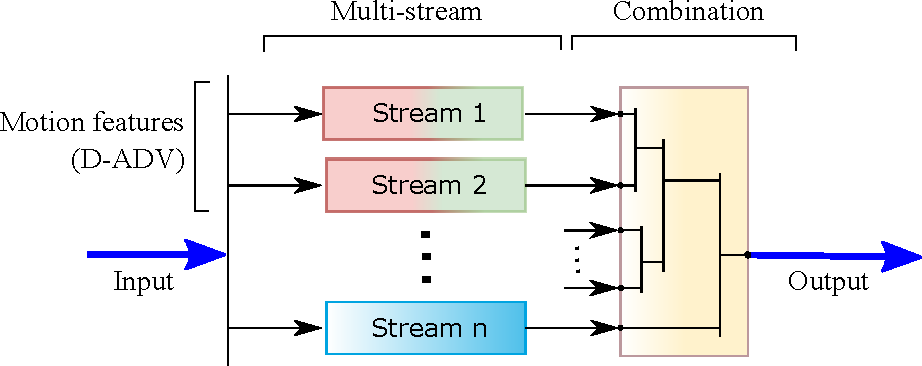
\includegraphics[width=\textwidth]{images/placeholder_figure.pdf}
  \caption{ROC per frame and $WS$=10}
  \label{fig:behave10f}
\end{subfigure}
~
\begin{subfigure}{0.5\textwidth}
  \centering
  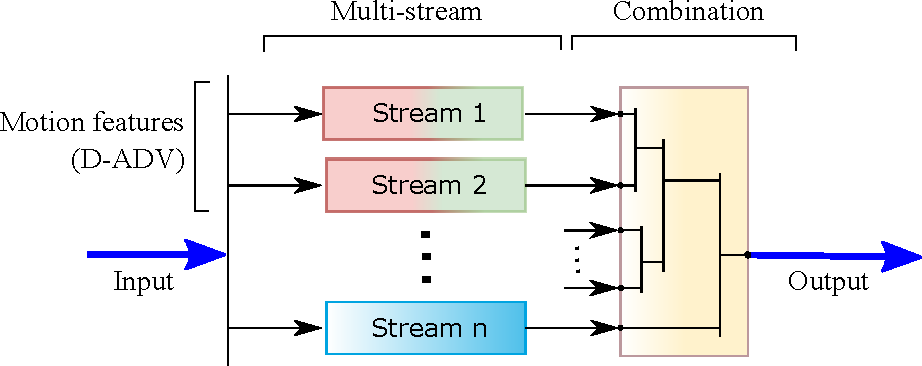
\includegraphics[width=\textwidth]{images/placeholder_figure.pdf}
  \caption{ROC per sequence and $WS$=10}
  \label{fig:behave10s}
\end{subfigure}
\\
\begin{subfigure}{0.5\textwidth}
  \centering
  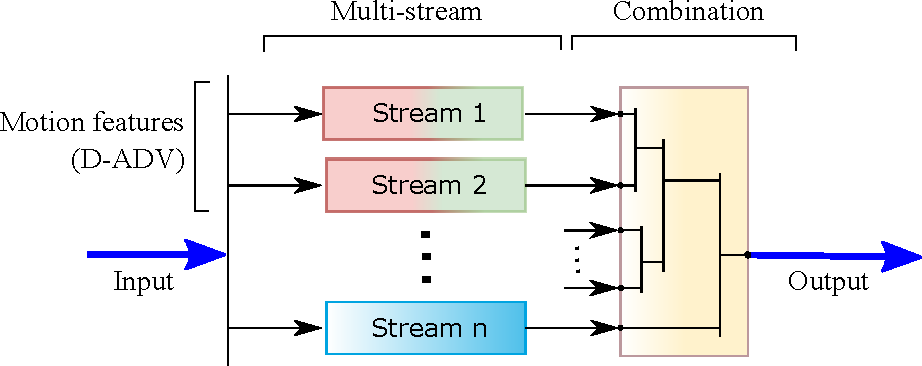
\includegraphics[width=\textwidth]{images/placeholder_figure.pdf}
  \caption{ROC per frame and $WS$=40}
  \label{fig:behave40f}
\end{subfigure}
~
\begin{subfigure}{0.5\textwidth}
  \centering
  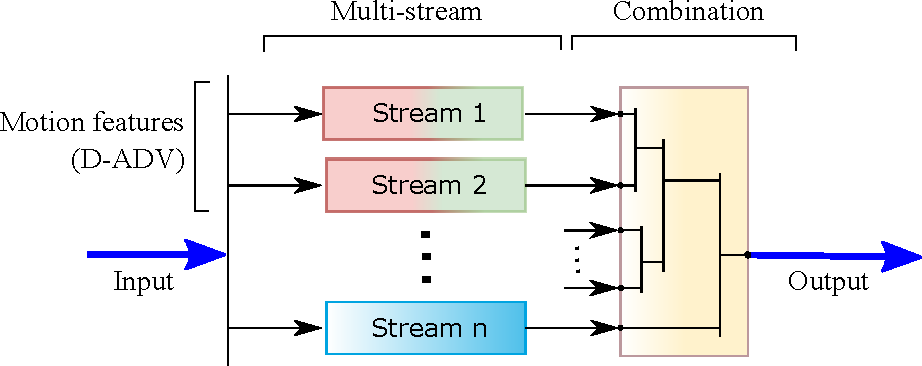
\includegraphics[width=\textwidth]{images/placeholder_figure.pdf}
  \caption{ROC per sequence and $WS$=40}
  \label{fig:behave40s}
\end{subfigure}
\caption{ROC curves for BEHAVE dataset}
\label{fig:fig_behave}
\end{figure*}

\begin{figure*}
\begin{subfigure}{0.5\textwidth}
  \centering
  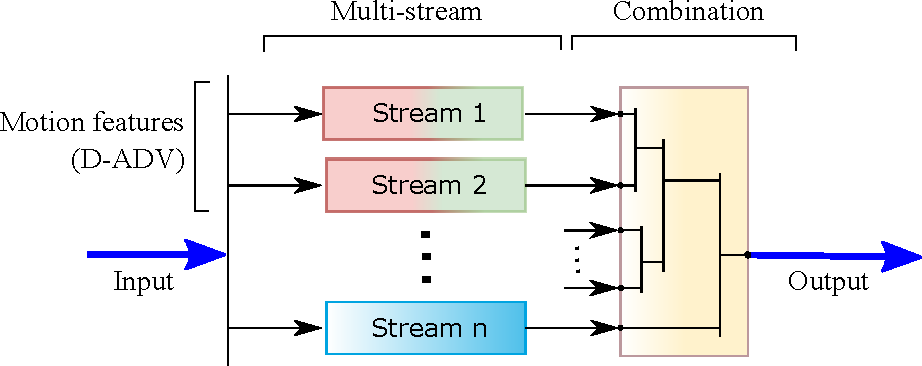
\includegraphics[width=\textwidth]{images/placeholder_figure.pdf}
  \caption{ROC per frame and $WS$=10}
  \label{fig:inria10f}
\end{subfigure}
~
\begin{subfigure}{0.5\textwidth}
  \centering
  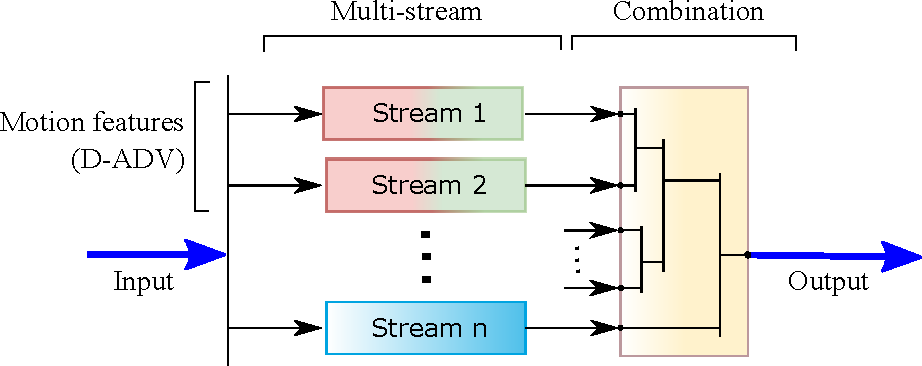
\includegraphics[width=\textwidth]{images/placeholder_figure.pdf}
  \caption{ROC per sequence and $WS$=10}
  \label{fig:inria10s}
\end{subfigure}
\\
\begin{subfigure}{0.5\textwidth}
  \centering
  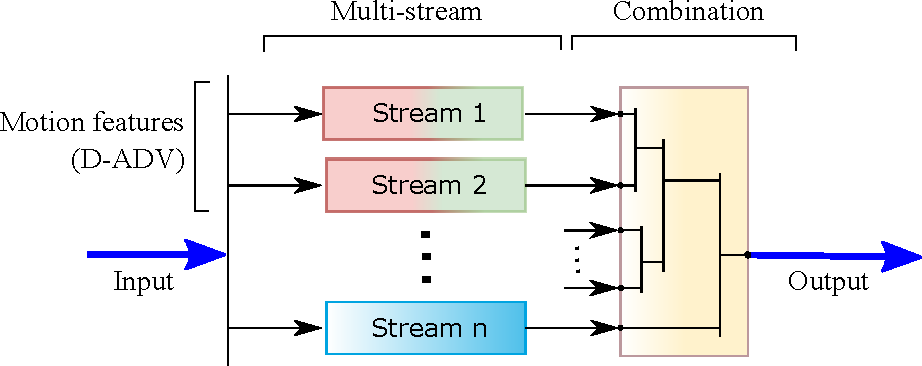
\includegraphics[width=\textwidth]{images/placeholder_figure.pdf}
  \caption{ROC per frame and $WS$=40}
  \label{fig:inria40f}
\end{subfigure}
~
\begin{subfigure}{0.5\textwidth}
  \centering
  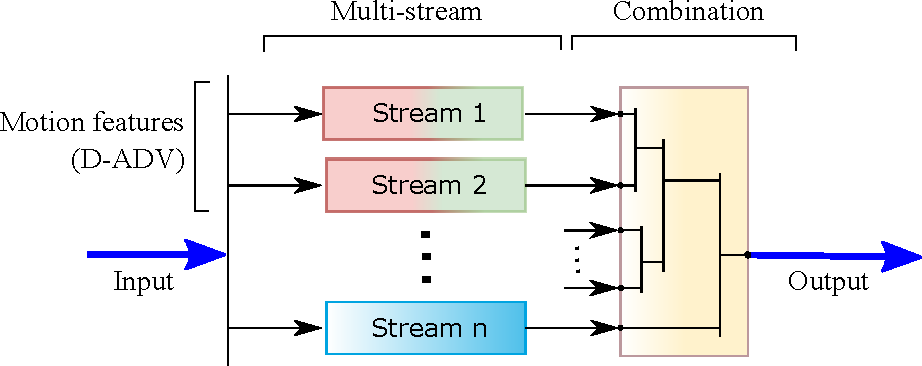
\includegraphics[width=\textwidth]{images/placeholder_figure.pdf}
  \caption{ROC per sequence and $WS$=40}
  \label{fig:inria40s}
\end{subfigure}
\caption{ROC curves for INRIA dataset}
\label{fig:fig_inria}
\end{figure*}

% Curvas ROC para CORRIDOR con windows size de 10 y 40
\begin{figure*}
	\begin{subfigure}{0.5\textwidth}		
	\centering
	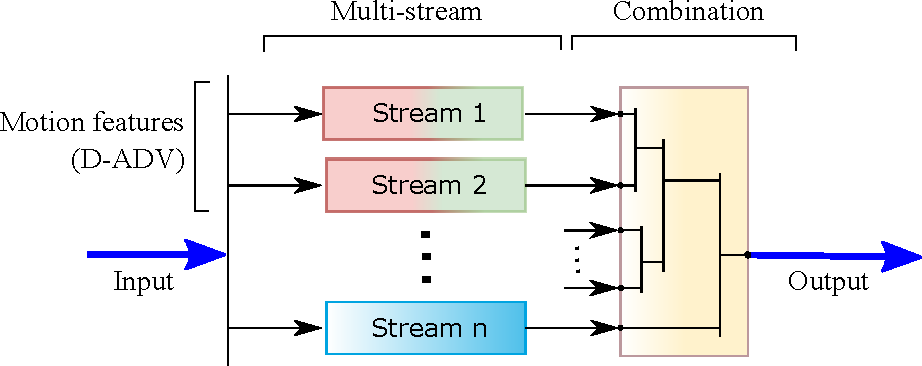
\includegraphics[width=0.9\textwidth]{images/placeholder_figure.pdf}
	\caption{ROC per frame and  $WS$= 10.}
	\label{fig:corridor-10-frame}
	\end{subfigure}
	~
	\begin{subfigure}{0.5\textwidth}		
	\centering
	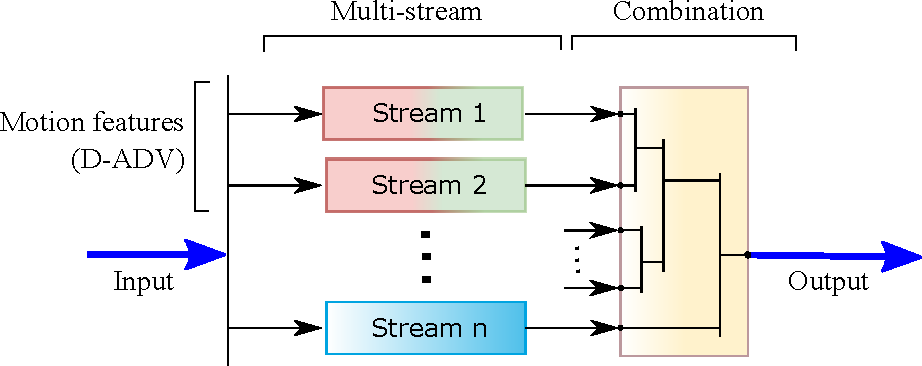
\includegraphics[width=0.9\textwidth]{images/placeholder_figure.pdf}
	\caption{ROC curves for CORRIDOR dataset and $WS$ = 10.}
	\label{fig:corridor-10-sequence}
	\end{subfigure}
	\\
	\begin{subfigure}{0.5\textwidth}
	\centering
	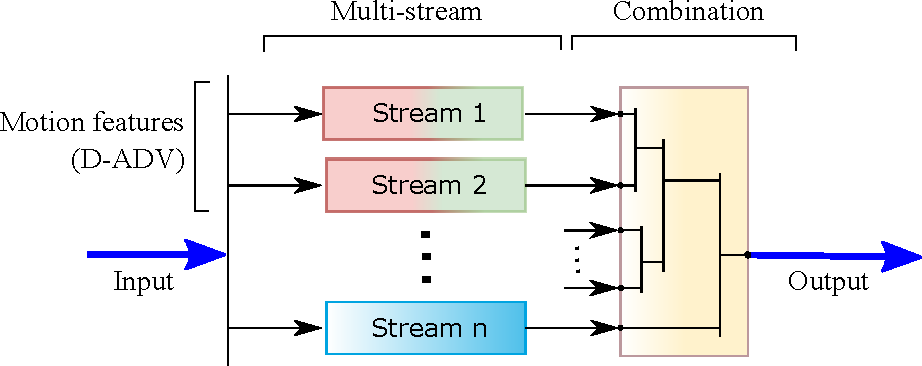
\includegraphics[width=0.9\textwidth]{images/placeholder_figure.pdf}
	\caption{ROC per frame and $WS$ = 40.}
	\label{fig:corridor-40-frame}
	\end{subfigure}
	~
	\begin{subfigure}{0.5\textwidth}
	\centering
	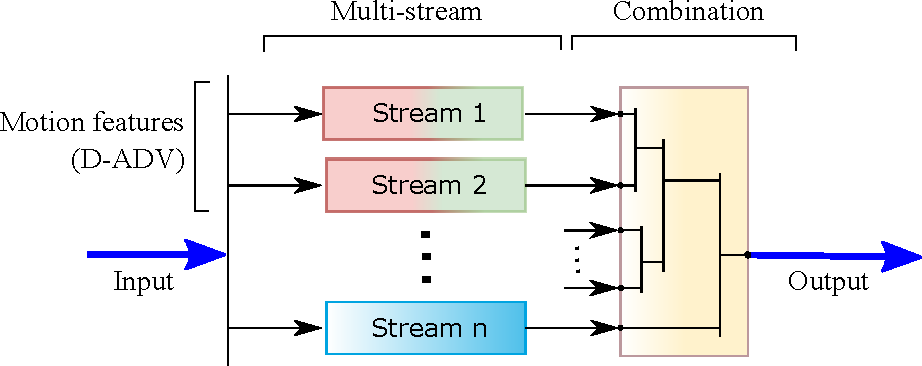
\includegraphics[width=0.9\textwidth]{images/placeholder_figure.pdf}
	\caption{ROC per sequence and $WS$ = 40.}
	\label{fig:corridor-40-seq}
	\end{subfigure}
	
	\caption{ROC curves for CORRIDOR dataset for frame and sequence with windosize parameter value of 10 and 40.}
	\label{fig:fig_corridor}
\end{figure*}

\begin{table*}[htbp]
  \centering
  \caption{Comparison according BEHAVE results}
    \resizebox{0.7\textwidth}{!}{\begin{tabular}{|l|rrrrrr|}
\cline{2-7}    \multicolumn{1}{r|}{} & \multicolumn{1}{l|}{D-ADV} & \multicolumn{1}{l}{GADV\cite{azorin2016}} & \multicolumn{1}{l}{\cite{cho2015group}} & \multicolumn{1}{l}{\cite{zhang2012recognizing}} & \multicolumn{1}{l}{\cite{munch2012supporting}} & \multicolumn{1}{l|}{\cite{yin2013small}} \\
    InGroup & 93,10\% & 86,67\% & 100,00\% & 88,00\% & 90,00\% & 94,30\% \\
    Approach & 93,94\% & 100,00\% & 83,33\% & 71,00\% & 60,00\% & -- \\
    Fight & 94,44\% & 90,00\% & 83,33\% &   --    &   --    & 95,10\% \\
    WalkTogether & 96,92\% & 86,67\% & 91,66\% & 88,00\% & 45,00\% & 92,10\% \\
    Split & 97,14\% & 100,00\% & 100,00\% & 79,00\% & 70,00\% & 93,10\% \\
    RunTogether & 100,00\% & 100,00\% & 83,33\% &   --    &   --    & -- \\
\cline{1-1}\cline{3-7}    Average & \textbf{95,93\%} & 93,89\% & 90,28\% & 81,50\% & 66,25\% & 93,65\% \\
    \hline
    \end{tabular}}%
  \label{tab:ComparisonBEHAVE}%
\end{table*}%


\subsection{One-Class}\label{sec:exp:oc}
The D-ADV-OC architecture has been evaluated using different instances. The simplest one is the \textit{D-ADV} instance that uses the original ADV descriptor \cite{azorin2014} with 15 x 15 cells followed by a fully connected layer of 15 x 15 x 5 neurons corresponding to the space of the ADV. The \textit{D-ADV+CNN} uses two Resnet50 neural networks to learn the LRF and UDF images without the top and the flatten layer connected to two concatenated 2D global average pooling layer (one per image stream) followed by a fully connected layer of 4096 neurons. Moreover, \textit{D-ADV+Context} and \textit{D-ADV+CNN+Context} uses the previous configurations with a third stream: the context recognition. In this case, a YOLO neural network trained with VOC has been used. The weights used for training are $w_a=0.9$ (activity) and $w_c=0.1$ (context). For all instances, two loss functions has been used: the OC-SVDD \cite{ruff2018deep} and the OC-NN \cite{chalapathy2018anomaly}. The window size ($ws$) as the number of consecutive frames considered in the accumulative process (see Figure \ref{fig:pipeline}) is 5 for the Ped1 and Avenue dataset and 10 for Ped2. Finally, the instances have been tested using the splits of training and tests predefined in the datasets.

The experimental results considering the sensitivity and the specificity as performance measure can be seen in Table \ref{tab:d-adv-oc}. As can be seen, high performances are obtained for all combinations in the different datasets. Having an average value in all cases higher than 70\% in all cases for both sensitivity and specificity, and reaching values on average close to 80\% for the D-ADV-Context instance with OC-SVDD. This configuration is the one that reaches the highest values for the Ped2 and Avenue datasets. Reaching close to 90\% in both parameters for Ped2. Although the configuration with OC-NN loss function has a very similar performance, it is in the Ped1 dataset where it achieves the best results. As for the use of the third stream with the Yolo object detection based context, it is shown that in all cases it improves the accuracy rates, avoiding a higher number of false alarms.

% Table generated by Excel2LaTeX from sheet 'Hoja1'
\begin{table*}
  \centering
  \caption{Results of the D-ADV-OC experiments for the PED 1, PED 2 and Avenue datasets. The OCC-SVDD and OCC-NN loss functions, with a combination of D-ADV, D-ADV+Context, D-ADV+CNN and D-ADV+CNN+Context classifiers are used to calculate sensitivity and specificity}
    \begin{tabular}{|c|l|r|r|r|r|r|r|r|r|}
\cline{3-10}    \multicolumn{1}{r}{} &       & \multicolumn{8}{c|}{Dataset} \bigstrut\\
\cline{3-10}    \multicolumn{1}{r}{} &       & \multicolumn{2}{c|}{Ped1} & \multicolumn{2}{c|}{Ped2} & \multicolumn{2}{c|}{Avenue} & \multicolumn{2}{c|}{All} \bigstrut\\
    \hline
    Instance & \multicolumn{1}{c|}{Loss func.} & \multicolumn{1}{c|}{Sens.} & \multicolumn{1}{c|}{Spec.} & \multicolumn{1}{c|}{Sens.} & \multicolumn{1}{c|}{Spec.} & \multicolumn{1}{c|}{Sens.} & \multicolumn{1}{c|}{Spec.} & \multicolumn{1}{c|}{Sens.} & \multicolumn{1}{c|}{Spec.} \bigstrut\\
    \hline
    \multirow{3}{*}{D-ADV} & OC-SVDD & 73,84\% & 73,87\% & 82,89\% & 82,87\% & 75,62\% & 75,62\% & 77,45\% & 77,45\% \bigstrut\\
\cline{2-10}          & OC-NN & 74,29\% & 74,20\% & 81,80\% & 81,77\% & 74,30\% & 74,29\% & 76,80\% & 76,75\% \bigstrut\\
\cline{2-10}          & Average & 74,07\% & 74,04\% & 82,35\% & 82,32\% & 74,96\% & 74,96\% & 77,12\% & 77,10\% \bigstrut\\
    \hline
    \multirow{3}{*}{\textbf{D-ADV+Context}} & OC-SVDD & 73,84\% & 73,87\% & \textbf{88,53\%} & \textbf{88,40\%} & \textbf{77,29\%} & \textbf{77,30\%} & \textbf{79,89\%} & \textbf{79,86\%} \bigstrut\\
\cline{2-10}          & OC-NN & \textbf{75,43\%} & \textbf{75,95\%} & 83,68\% & 83,15\% & 75,57\% & 75,17\% & 78,23\% & 78,09\% \bigstrut\\
\cline{2-10}          & Average & 74,64\% & 74,91\% & 86,11\% & 85,78\% & 76,43\% & 76,24\% & 79,06\% & 78,97\% \bigstrut\\
    \hline
    \multirow{3}{*}{D-ADV+CNN} & OC-SVDD & 69,74\% & 69,73\% & 71,36\% & 71,27\% & 71,63\% & 71,61\% & 70,91\% & 70,87\% \bigstrut\\
\cline{2-10}          & OC-NN & 68,90\% & 68,94\% & 73,24\% & 73,20\% & 73,36\% & 73,35\% & 71,83\% & 71,83\% \bigstrut\\
\cline{2-10}          & Average & 69,32\% & 69,34\% & 72,30\% & 72,24\% & 72,50\% & 72,48\% & 71,37\% & 71,35\% \bigstrut\\
    \hline
    \multirow{3}{*}{D-ADV+CNN+Context} & OC-SVDD & 70,31\% & 70,30\% & 85,19\% & 85,64\% & 71,93\% & 71,87\% & 75,81\% & 75,94\% \bigstrut\\
\cline{2-10}          & OC-NN & 69,84\% & 69,84\% & 74,27\% & 74,31\% & 74,35\% & 74,34\% & 72,82\% & 72,83\% \bigstrut\\
\cline{2-10}          & Average & 70,08\% & 70,07\% & 79,73\% & 79,98\% & 73,14\% & 73,11\% & 74,32\% & 74,38\% \bigstrut\\
    \hline
    \end{tabular}%
  \label{tab:d-adv-oc}%
\end{table*}%


Finally, the experimental results are showed and compared with other state-of-the-art methods in Table \ref{tab:occ-ped-avenue} at frame-level. Results for the UCSD Ped 1 dataset show that the lowest value of EER is 23.50\% provided in the work by Vu et al. \cite{vu2019robust} and the highest AUC value is 86.26\% in the work by Lu et al. \cite{lu2019future}. According to EER for the UCSD Ped2 dataset, the best results (4.68\%) are obtained again in the work by Vu et al. However in AUC, the maximum value is achieved by Ionescu et al. \cite{ionescu2019object} (97.80%). For the Avenue, the best AUC is again for the work by Ionescu et al. (90.40\%) and the best EER for other work proposed by Li et al. \cite{li2019spatio} (21.50%). Our proposed architecture with the different instances is not the best for any dataset but the performance is in accordance with those obtained in the other works. As can be seen, if we compare our work with the average results obtained by the state-of-the-art works, it improves in all cases except for Avenue's AUC (our work achieves ~82\% compared to an average of ~83\%). The best configurations for AUC and EER are with the \textit{D-ADV+Context} configuration and with a loss function OC-NN for Ped1 and Avenue, and OC-SVDD for Ped2. 

\begin{table*}
	\centering
	\caption{Comparison of D-ADV-OC results at frame level with other methods with PED 1, PED 2 and Avenue datasets. Cells containing the letters ND indicate that no data is available.}
	\label{tab:occ-ped-avenue}
	\resizebox{0.49\textwidth}{!}{\begin{tabular}{l|c|c|c|c|c|c|}
	\cline{2-7}
	& \multicolumn{6}{c|}{\textbf{Frame level}} \\ \cline{2-7} 
	& \multicolumn{2}{c|}{\textbf{Ped 1}} & \multicolumn{2}{c|}{\textbf{Ped 2}} & \multicolumn{2}{c|}{\textbf{Avenue}} \\ \hline
	\multicolumn{1}{|c|}{\textbf{Reference}} & \textbf{AUC \%} & \textbf{EER \%} & \textbf{AUC \%} & \textbf{EER \%} & \textbf{AUC \%} & \textbf{EER \%} \\ \hline
	\multicolumn{1}{|c|}{\cite{vu2019robust}} & 82.34 & 23.50 & 97.52 & 4.68 & 71.54 & 36.38 \\ \hline
	\multicolumn{1}{|c|}{\cite{hu2019efficient}} & 80.90 & 26.30 & 95.90 & 10.50 & 84.20 & 23.00 \\ \hline
	\multicolumn{1}{|c|}{\cite{zhou2019anomalynet}} & 83.50 & 25.20 & 94.90 & 10.30 & 86.10 & 22.00 \\ \hline
	\multicolumn{1}{|c|}{\cite{li2019spatio}} & 83.80 & 22.30 & 96.50 & 8.70 & 84.50 & 21.50 \\ \hline
	\multicolumn{1}{|c|}{\cite{wang2018detecting}} & 77.80 & 29.20 & 96.40 & 8.90 & 85.30 & 23.90 \\ \hline
	\multicolumn{1}{|c|}{\cite{ribeiro2018study}} & 53.50 & 48.00 & 81.40 & 26.00 & 73.80 & 32.80 \\ \hline
	\multicolumn{1}{|c|}{\cite{lee2018stan}} & 82.10 & ND & 96.50 & ND & 87.20 & ND \\ \hline
	\multicolumn{1}{|c|}{\cite{lu2019future}} & 86.26 & ND & 96.06 & ND & 85.78 & ND \\ \hline
	\multicolumn{1}{|c|}{\cite{ionescu2019object}} & ND & ND & 97.80 & ND & 90.40 & ND \\ \hline
	\multicolumn{1}{|c|}{\cite{nguyen2019anomaly}} & ND & ND & 96.20 & ND & 86.90 & ND \\ \hline
	\multicolumn{1}{|c|}{\cite{ye2019anopcn}} & ND & ND & 96.80 & ND & 86.20 & ND \\ \hline
	\multicolumn{1}{|c|}{\cite{nguyen2019hybrid}} & ND & ND & 82.80 & ND. & 84.30 & ND \\ \hline
	\multicolumn{1}{|c|}{\textbf{Average}} & \multicolumn{1}{c|}{\textbf{78.78}} & \multicolumn{1}{|c|}{\textbf{29.08}} & \multicolumn{1}{c|}{\textbf{94.07}} & \multicolumn{1}{c|}{\textbf{11.51}} & \multicolumn{1}{c|}{\textbf{83.85}} & \multicolumn{1}{c|}{\textbf{26.60}} \\ \hline
	\multicolumn{1}{|c|}{\textbf{Proposed}} & \multicolumn{1}{c|}{\textbf{84.41}} & \multicolumn{1}{|c|}{\textbf{24.36}} & \multicolumn{1}{c|}{\textbf{95.04}} & \multicolumn{1}{c|}{\textbf{11.49}} & \multicolumn{1}{c|}{\textbf{82.29}} & \multicolumn{1}{c|}{\textbf{22.70}} \\
	\multicolumn{1}{|c|}{\textbf{Architecture}} & \multicolumn{1}{l|}{} & \multicolumn{1}{l|}{} & \multicolumn{1}{l|}{} & \multicolumn{1}{l|}{} & \multicolumn{1}{l|}{} & \multicolumn{1}{l|}{} \\
	\hline
	\end{tabular}}
\end{table*}
